\documentclass{standalone}
\usepackage{tikz}
\usetikzlibrary{positioning}
\usetikzlibrary{calc}
\usetikzlibrary{fit}
\usetikzlibrary{shapes}
\usetikzlibrary{arrows}
\usetikzlibrary{intersections}

\tikzset{>=latex}
\tikzset{transaction/.style={font=\small{#1}}}
\tikzset{key/.style={rectangle, draw, minimum height=10pt, text width=2cm, align=center}}
\tikzset{hash/.style={rectangle, draw, minimum height=10pt, text width=1cm, align=center}}
\tikzset{signature/.style={rectangle, draw, minimum height=10pt, text width=2cm, align=center}}

\tikzset{block/.style={font=\small{#1}}}
\tikzset{blockheader/.style={font=\small{#1}}}
\tikzset{field/.style={rectangle, draw, minimum height=10pt, text width=2cm, align=center}}
\tikzset{hash/.style={rectangle, dashed, draw, minimum height=10pt, text width=1.2cm, align=center}}
\tikzset{tx/.style={rectangle, draw, minimum height=10pt, text width=2cm, align=center}}


\begin{document}
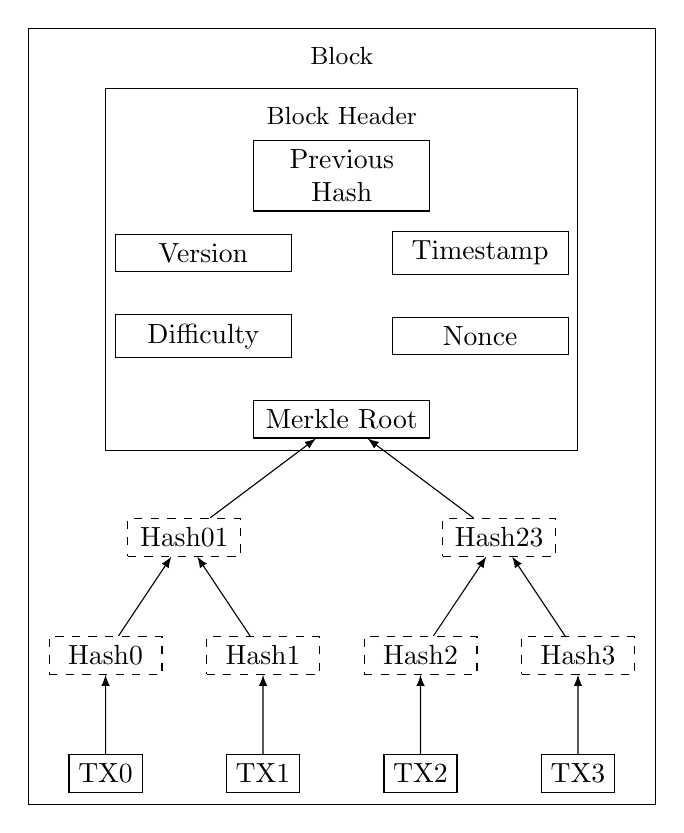
\begin{tikzpicture}[remember picture, every node/.style={},
        level 1/.style={sibling distance=40mm},
        level 2/.style={sibling distance=20mm},
        edge from parent/.style={draw,latex-}
    ]
    \node [block] (b0) at (20,20) {Block};
    \node [blockheader] (h0) at ($(b0.south) + (0,-15pt)$) {Block Header};
    \node [field] (prevHash0) at ($(h0.south) + (0,-15pt)$) {Previous Hash};

    \node [field] (version0) at ($(prevHash0.south) + (-50pt,-15pt)$) {Version};
    \node [field] (timestamp0) at ($(prevHash0.south) + (50pt,-15pt)$) {Timestamp};

    \node [field] (difficulty0) at ($(version0) + (0,-30pt)$) {Difficulty};
    \node [field] (nonce0) at ($(timestamp0) + (0,-30pt)$) {Nonce};

    \node [field] (merkleRoot0) at ($(nonce0) + (-50pt,-30pt)$) {Merkle Root}
        child {node [hash] {Hash01}
            child {node [hash] (hash0) {Hash0}
                child {node [grow=down, draw] (tx0) {TX0}}
            }
            child {node [hash] {Hash1}
                child {node [grow=down, draw] {TX1}}
            }
        }
        child {node [hash] {Hash23}
            child {node [hash] {Hash2}
                child {node [grow=down, draw] {TX2}}
            }
            child {node [hash] (hash3) {Hash3}
                child {node [grow=down, draw] {TX3}}
            }
        };

     % The border surrounding the block header.
    \node (hb0) [draw=black, fit={(h0) (version0) (timestamp0) (difficulty0)
        (nonce0) ($(prevHash0.south) - (0,1pt)$)
        ($(merkleRoot0.south) - (0,1pt)$)}] {};

     % The border surrounding the entire block.
    \node (bb0) [draw=black, fit={(b0) ($(hash0.west) - (4pt,0)$)
        ($(hash3.east) + (4pt,0)$) ($(tx0.south) - (0,1pt)$)}] {};

\end{tikzpicture}
\end{document}
